\subsection*{OBROK '19 aneb LEMŠEŘÍ VÝLET NA KONOPIŠTĚ}
\label{sub:obrok19}

Už na samotný počátek byl napínavý - masivní přihlašování je vždycky otázkou rychlosti, takže jsme všichni, kdo chtěli jet na ObRok, seděli u svých počítačů/mobilů, netrpělivě odpočítávali poslední minuty a celí nervózní čekali, až se v osm večer spustí přihlašování. Samozřejmě, servery padaly a ne všichni se dostaly hned na poprvé. Naštěstí ale ještě poté byla druhá vlna přihlašování, takže jsme nakonec (přes menší komplikace v podobě nemocí, doplňování členů apod.) na akci jeli ve složení Tarzan - jako vedoucí naší skupiny, Koala, Šárka, Wexlák, Kibitz, Šerif, Natěrač, já a pak ještě další tři skauti z Tábora - Ponožka  a jeho dvě ženy :).


ObRok jako takový se konal na Konopišti nedaleko Benešova u Prahy. Už při příchodu jsme poznali, že tu jsou opravdu lidé z různých krajů - zpívající Ostravaci se nedali přeslechnout. Bohužel, počasí nám ze začátku příliš nepřálo. Pršelo, pršelo a pršelo, což nakonec mělo dopad i na celý ObRok, kdy jsme ze subkempů museli poměrně dlouhou cestou obcházet obrokový areál, abychom se vůbec dostali k pódiu a dalším stánkům, neboť původní cesta byla velmi rozbahněná. Takže jsme často na různé ceremonie, programy a koncerty chodili později, než bychom si přáli.

\begin{center}
	
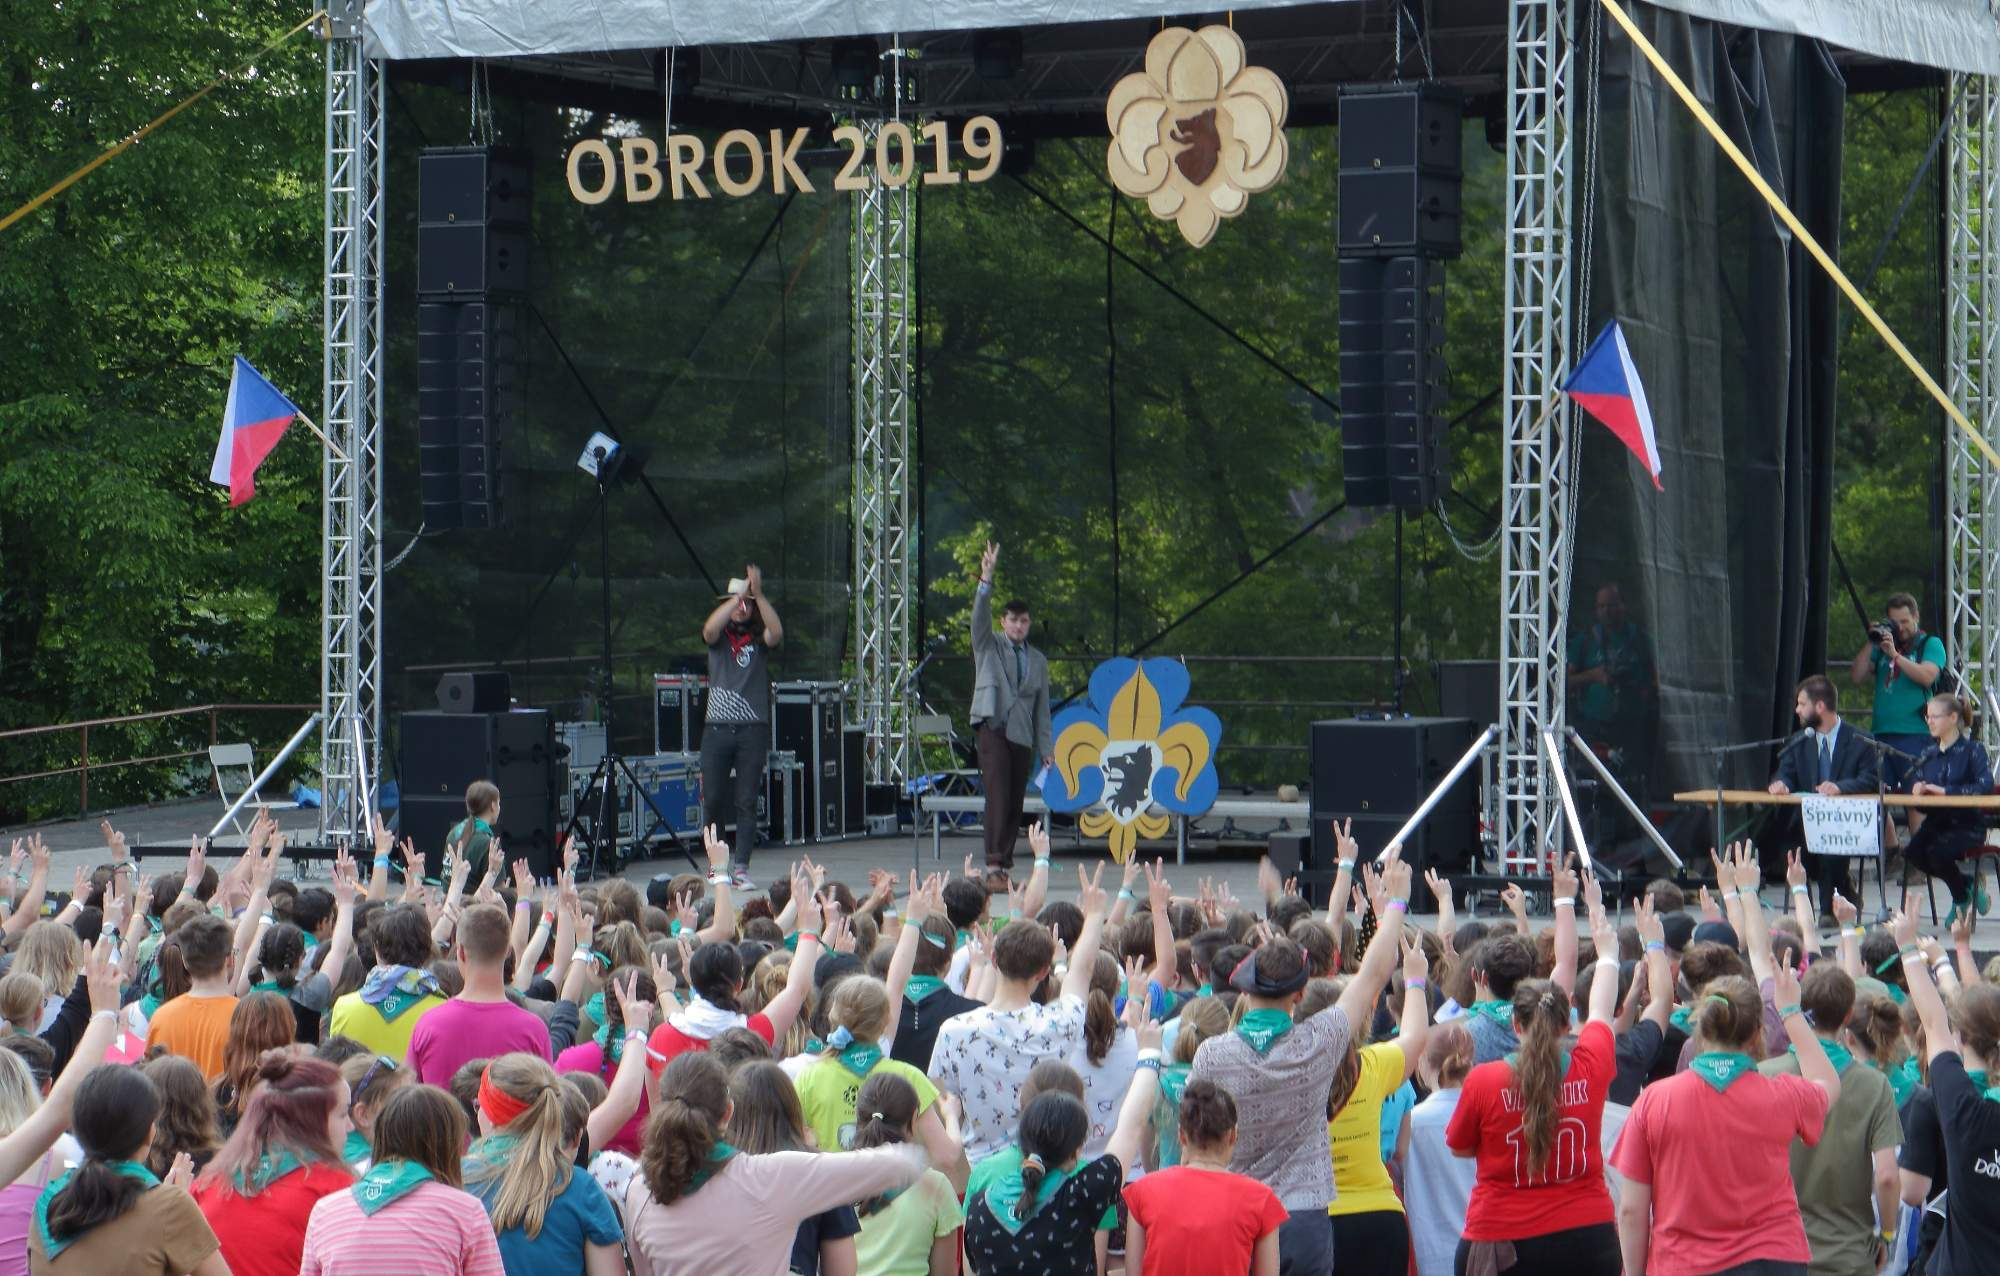
\includegraphics[width=12cm]{img/rovero_clanky/obrok1.JPG}
\end{center}

Programů tam bylo požehnaně - různé workshopy, služby, velká hra, koncerty, netradiční sporty, přednášky… člověk se tam opravdu nenudil. Ovšem vzhledem k té obrovské mase lidí bylo kolikrát těžké se někam dostat. Mě osobně nejvíce bavilo sobotní odpoledne, kdy jsme šli službit jako pomocníci při dětském dopravním dni pro benešovské. Byla jsem tam s moc fajn lidmi a potkala jsem spoustu jak roztomilých, tak vtipných dětí. Celkově zajímavá zkušenost. A samozřejmě jsem si užila koncerty (kapela Skaunk a frontman kapely Mech budiž navždy uchováni v mém srdíčku)!
Také mě pobavilo hromadné koukání na hokej v kantýně. Protože i když byl člověk na druhém konci areálu, poznal, že Češi dali puk.


Co se týče jídla, tak to se mnou bylo docela problematické. Kvůli různým problémům mi bylo od doktorky nakázáno nepožívat lepek a laktózu, takže původně velmi solidní výběr potravin se drasticky snížil na luštěniny, ovoce, zeleninu, rýži a maso. Takže si to se mnou vařící Přííšery jistě užily :). Tak či tak jsme ale vykouzlily moc dobré menu.


Jeden pro mě z mála nepříjemných okamžiků, jež se na ObRoku staly, se přihodil při velké obrokové hře - kolínko šlo do háje, což jemně zkomplikovalo náš odjezd. Díky mně jsme totiž kráčeli celkem pomalu a připočítáme-li ještě zapomenutý kotlík a České dráhy, výsledkem byla další společná a krásně strávená chvíle - čekání na vlak. Naštěstí jsme se ale všichni dostali domů relativně včas.


Závěrem bych celou akci zhodnotila pozitivně. Sice jsem si tam nenašla moc nových kamarádů, ale za to jsem si to užila s těmi starými! A věřím, že ostatní Lemšery taky!


\begin{center}

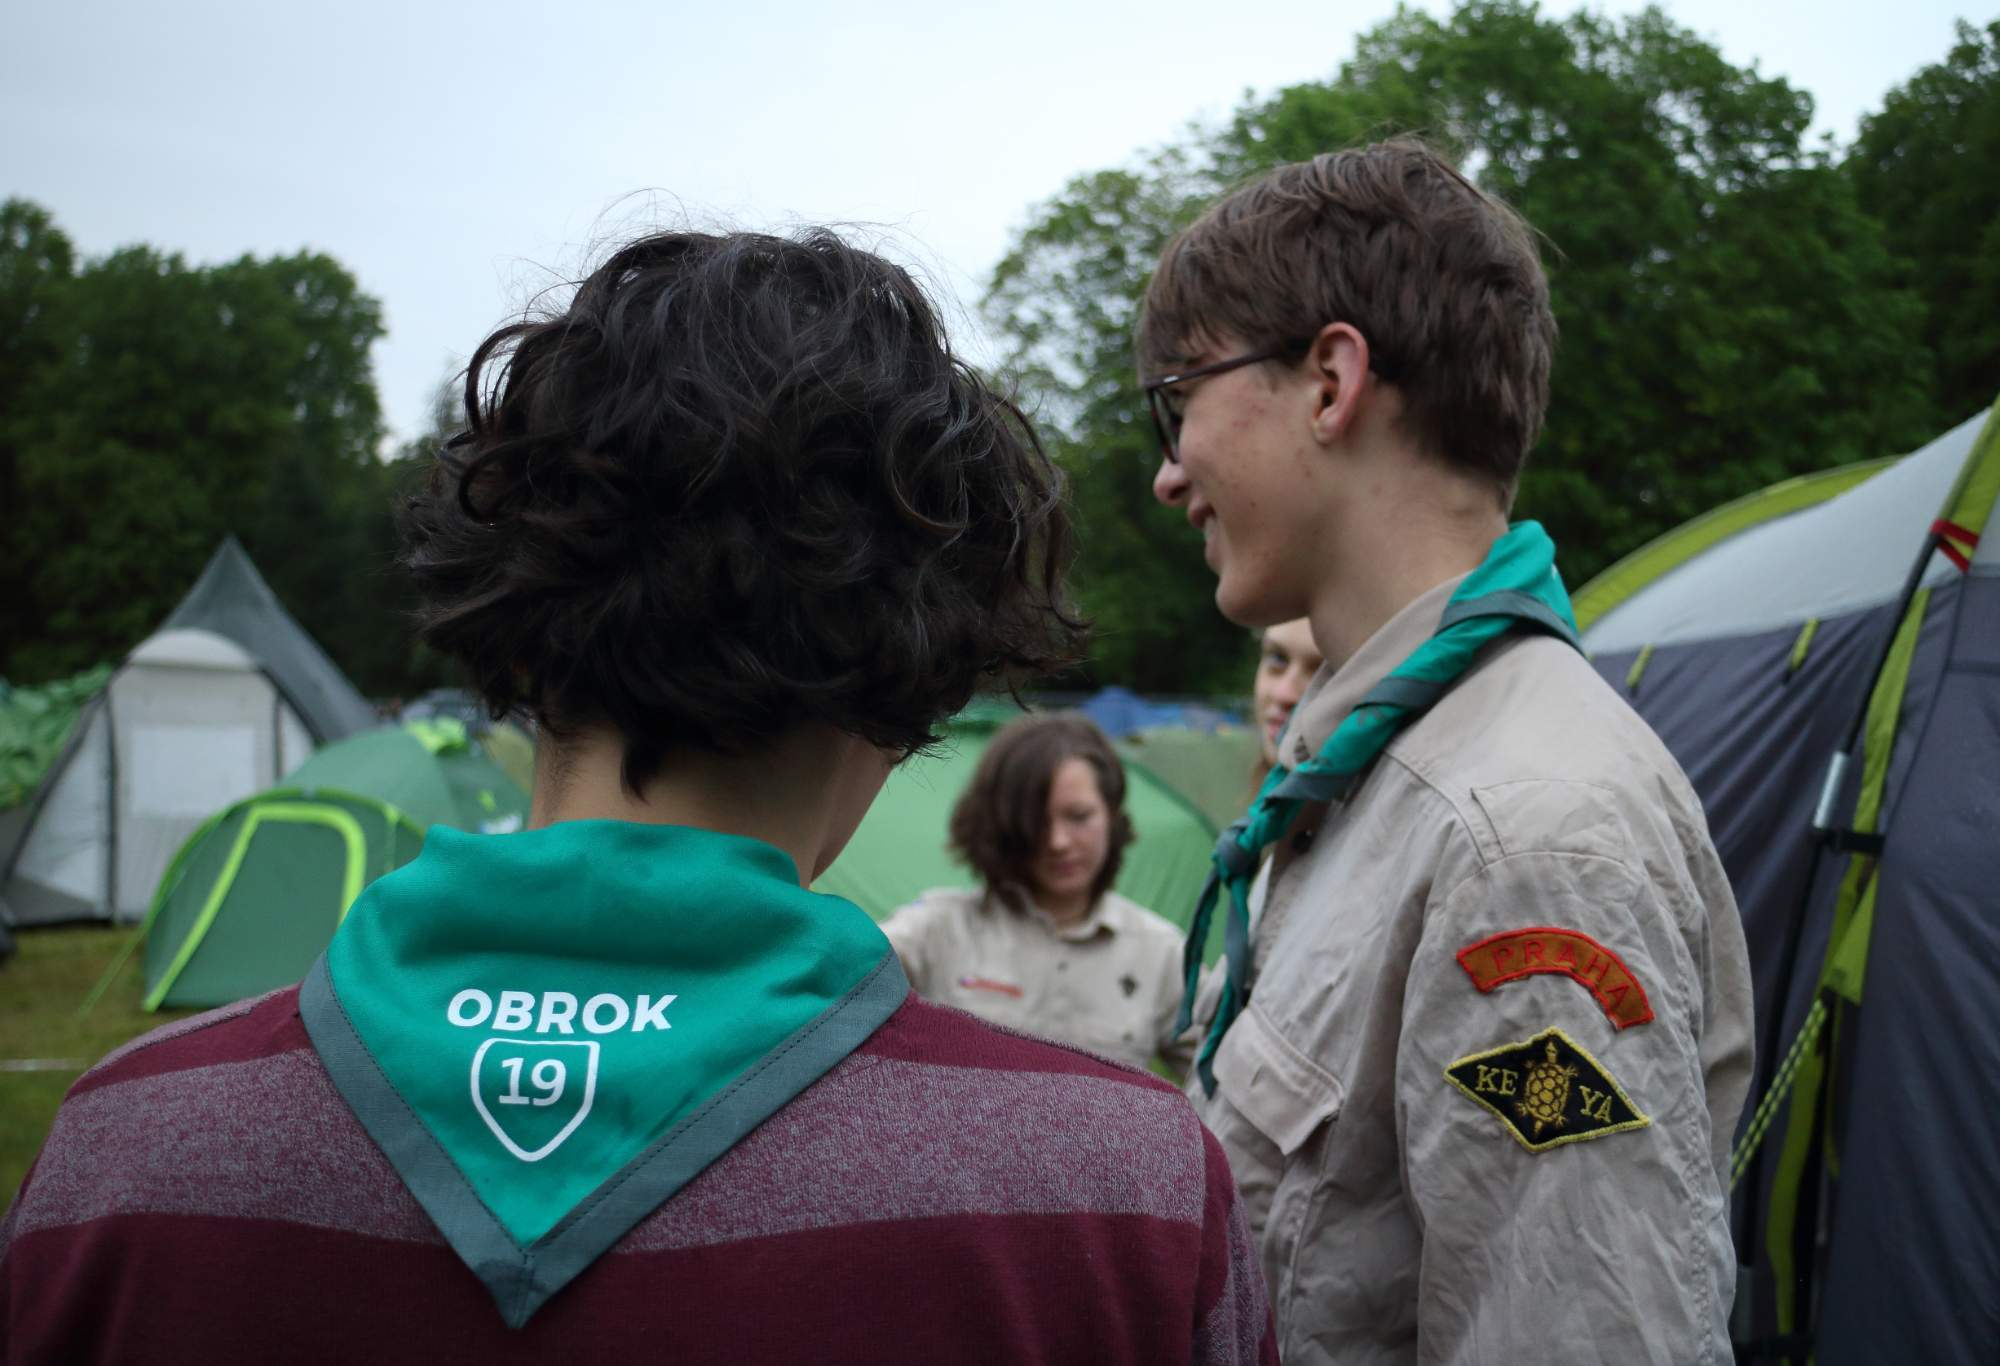
\includegraphics[width=12cm]{img/rovero_clanky/obrok2.JPG}

\end{center}


\podpis{Štípadlo}